\documentclass[article]{jss}
\usepackage[utf8]{inputenc}

\providecommand{\tightlist}{%
  \setlength{\itemsep}{0pt}\setlength{\parskip}{0pt}}

\author{
Derek Corcoran\\University of Missouri \And Elisabeth Webb\\University of Missouri, USGS \And Dylan Kesler\\Institute Of Bird Population
}
\title{Selecting priority areas from diversity and individual species abundance
\pkg{DiversityOccupancy}}
\Keywords{\pkg{DiversityOccupancy}, Occupancy Modeling, \proglang{R}}

\Abstract{
Lately occupancy modeling has been vastly used as a tool for ecological
research and management planing. However mostly it is used by
interpreting single species models. We present the
\pkg{DiversityOccupancy} in the \proglang{R} environment. The objective
of this package is to simultaneously model factors associated with
occupancy and abundance of individual species using a detection history
file, and to use predicted abundances to calculate species diversity for
each sampling site. The package then models factor(s) associated with
among-site species diversity, which can then be combined with spatial
data to identify areas that contain both high abundance of species of
conservation concern and high species diversity.
}

\Plainauthor{Derek Corcoran, Elisabeth Webb, Dylan Kesler}
\Shorttitle{\pkg{DiversityOccupancy}: Selecting Priority Areas}
\Plainkeywords{keywords, not capitalized, Occupancy modeling}

%% publication information
%% \Volume{50}
%% \Issue{9}
%% \Month{June}
%% \Year{2012}
\Submitdate{}
%% \Acceptdate{2012-06-04}

\Address{
    Derek Corcoran\\
  University of Missouri\\
  First line Second line\\
  E-mail: \href{mailto:corcoranbarriosd@missouri.edu}{\nolinkurl{corcoranbarriosd@missouri.edu}}\\
  URL: \url{http://rstudio.com}\\~\\
      }

\usepackage{amsmath}

\begin{document}

\section{Introduction}\label{introduction}

In the last decade, Occupancy modeling has been used more and more as a
method to account for how species respond to environmental or
anthropogenic factors. It has also been shown to be useful as a species
distribution modeling tool when species have imperfect detection
\cite{mackenzie_estimating_2002}. Anthore use for what it has been used
is for managers to change the environment of managed areas in order to
improve the status of species of conservation concern. Unfortunantely
this decision usually comes without taking into account the effect of
such management action on species diversity. There has been several
authors championing for the use of species specific or diversity related
approaches to plan conservation issues, but as far as we know this is
the first method that takes into account both species diversity and
individual species abundance in order to select conservation areas.

\subsection{Installing
DiversityOccupancy}\label{installing-diversityoccupancy}

\subsubsection{Requirements}\label{requirements}

To use this package you need \proglang{R} version 3.2.2 or newer (use
the function \code{sessionInfo()} in your R session to check your
current version).

\subsubsection{Installing the package}\label{installing-the-package}

Install from cran repository

\begin{CodeChunk}
\begin{CodeInput}
install.packages("DiversityOccupancy")
\end{CodeInput}
\end{CodeChunk}

\subsection{Objectives of the Package}\label{objectives-of-the-package}

The objective of this package is to simultaneously model factors
associated with occupancy and abundance of individual species using a
detection history file, and to use predicted abundances to calculate
species diversity for each sampling site. The package then models
factor(s) associated with among-site species diversity, which can then
be combined with spatial data to identify areas that contain both high
abundance of species of conservation concern and high species diversity.

\subsection{Use of the package}\label{use-of-the-package}

In order to calculate abundance and alpha diversity we need at least
three files:

\paragraph{Detection history of multiple
species}\label{detection-history-of-multiple-species}

A data frame consisting on the detection history of at least two
species. As an example \pkg{DiversityOccupancy} has the data-set BatOccu
which contains detection histories of 17 species of bats in the Plumas
National Forest for 3 consecutive days (Columns) in 49 different sites
(Rows). The data set includes a 1 for each time a species was detected,
and a 0 for each time it was not detected.

A detection for the first three species is presented below:

\begin{CodeChunk}
\begin{CodeInput}
library(DiversityOccupancy)
data("BatOccu")
head(BatOccu[1:9])
\end{CodeInput}
\begin{CodeOutput}
  Myyu1 Myyu2 Myyu3 Myca1 Myca2 Myca3 Myci1 Myci2 Myci3
1     0     0     0     0     0     0     0     0     0
2     1     0     0     1     0     0     0     0     0
3     0     0     0     0     1     0     0     0     0
4     0     0     0     0     0     0     0     0     0
5     0     0     0     1     1     1     0     0     0
6     1     0     0     1     1     1     0     0     0
\end{CodeOutput}
\end{CodeChunk}

\paragraph{Site covariates}\label{site-covariates}

Site covariates are presented in a data frame consisting of measurements
taken at each site. The covariates are used singly and in combination to
model occupancy or abundance, and they should be variables that are
stable within the scope of the length of the study. In
\pkg{DiversityOccupancy} there is an example concordant with the BatOccu
data set called sampling.cov:

\begin{CodeChunk}
\begin{CodeInput}
data("sampling.cov")
head(sampling.cov)
\end{CodeInput}
\end{CodeChunk}

\begin{CodeChunk}
\begin{CodeOutput}
  Distance.to.water Distance.to.road Existing.vegetation Fire.Interval
1                 0         325.2647            3.000000      14.79164
2                 0           0.0000           15.294588      11.00000
3                 0           0.0000            4.769200      16.00000
4                 0           0.0000            4.705464      18.27010
5                 0           0.0000           14.224747      14.97247
6                 0        2308.6010           15.727460      15.81841
  Altitude Burn.intensity.soil Burn.intensity.Canopy Burn.intensity.basal
1 1859.337          0.00000000            0.00000000           0.00000000
2 1839.813          0.24802029            0.12812701           0.12812701
3 1890.586          0.00000000            0.00000000           0.00000000
4 1927.237          0.00000000            0.00000000           0.00000000
5 1682.559          3.42075635            3.84151252           5.30799686
6 1515.009          0.01135227            0.01135223           0.01135223
\end{CodeOutput}
\end{CodeChunk}

\paragraph{Detection covariates}\label{detection-covariates}

A list of data frames, in which each data frame includes a daily
measurement of variables with the potential to affect detection
probabilities. It is important that each element (data frame) of the
list has a name, so that it can be called to fit the occupancy model.
These variables are used to model the probability of detection.

\pkg{DiversityOccupancy} has a data set called \emph{Dailycov} which
illustrates how the Daily covariates have to be structured:

\begin{CodeChunk}
\begin{CodeInput}
#All the items of the ist must have names
names(Dailycov)
\end{CodeInput}
\begin{CodeOutput}
[1] "Julian"   "Maxhum"   "Maxtemp"  "Meanhum"  "Meantemp" "Minhum"  
[7] "Mintemp"  "sdhum"    "sdtemp"  
\end{CodeOutput}
\begin{CodeInput}
#here we see the first dataframe of the Dailycov dataset
head(Dailycov[[1]])
\end{CodeInput}
\begin{CodeOutput}
  Julian.Julian1 Julian.Julian2 Julian.Julian3
1      -1.683391      -1.683391      -1.683019
2      -1.620723      -1.620723      -1.620362
3      -1.684443      -1.684443      -1.684071
4      -1.557310      -1.557310      -1.556958
5      -1.429475      -1.429475      -1.434405
6      -1.241253      -1.241253      -1.240951
\end{CodeOutput}
\end{CodeChunk}

\subsection{Fiting models for abundance and predicting alpha
diversity}\label{fiting-models-for-abundance-and-predicting-alpha-diversity}

In this example we will fit and model the abundance for 17 bat species
and calculate alpha diversity from those results.

\begin{CodeChunk}
\begin{CodeInput}
BatDiversity <-diversityoccu(pres = BatOccu, sitecov = sampling.cov, obscov =
Dailycov,spp = 17, form = ~ Julian + Meanhum ~ Burn.intensity.soil +
I(Burn.intensity.soil^2), dredge = FALSE)
\end{CodeInput}
\end{CodeChunk}

The resulting object of class diversityoccupancy has the following
elements

\begin{CodeChunk}
\begin{CodeInput}
names(BatDiversity)
\end{CodeInput}
\begin{CodeOutput}
[1] "Covs"      "models"    "Diversity" "species"  
\end{CodeOutput}
\end{CodeChunk}

If you need to see the parameters of the model of one of the species,
you call the species number with the element\$models. For example
extract the model for the second species:

\begin{CodeChunk}
\begin{CodeInput}
BatDiversity$models[[2]]
\end{CodeInput}
\begin{CodeOutput}

Call:
occuRN(formula = form, data = models[[i]])

Abundance:
                          Estimate     SE      z P(>|z|)
(Intercept)               0.000567 0.2829  0.002   0.998
Burn.intensity.soil       0.543374 0.3826  1.420   0.156
I(Burn.intensity.soil^2) -0.092936 0.0996 -0.933   0.351

Detection:
            Estimate    SE      z P(>|z|)
(Intercept)    0.113 0.357  0.317  0.7512
Julian        -0.097 0.267 -0.364  0.7159
Meanhum       -0.548 0.246 -2.228  0.0259

AIC: 180.113 
\end{CodeOutput}
\end{CodeChunk}

The species parameter for a diversityoccupancy object shows us a table with the abundance and alpha diversity calculated for each sampled point:

\begin{CodeChunk}
\begin{CodeInput}
summary(BatDiversity$species)
\end{CodeInput}
\begin{CodeOutput}
       h           species.1        species.2       species.3     
 Min.   :2.115   Min.   :0.3528   Min.   :1.001   Min.   :0.1156  
 1st Qu.:2.115   1st Qu.:0.3528   1st Qu.:1.001   1st Qu.:0.1156  
 Median :2.277   Median :0.5153   Median :1.300   Median :0.1883  
 Mean   :2.291   Mean   :0.7520   Mean   :1.523   Mean   :0.3401  
 3rd Qu.:2.488   3rd Qu.:1.2428   3rd Qu.:2.045   3rd Qu.:0.6356  
 Max.   :2.553   Max.   :1.3027   Max.   :2.214   Max.   :0.6695  
   species.4        species.5        species.6           species.7     
 Min.   :0.4802   Min.   :0.3020   Min.   :0.0000223   Min.   : 2.776  
 1st Qu.:0.5504   1st Qu.:0.3020   1st Qu.:0.0000223   1st Qu.: 4.261  
 Median :0.5863   Median :0.5035   Median :0.0004349   Median : 6.424  
 Mean   :0.6125   Mean   :0.6907   Mean   :0.0983938   Mean   : 6.267  
 3rd Qu.:0.5870   3rd Qu.:1.1210   3rd Qu.:0.1874298   3rd Qu.: 6.424  
 Max.   :0.8884   Max.   :1.2776   Max.   :0.3654810   Max.   :12.836  
   species.8       species.9        species.10       species.11    
 Min.   :1.716   Min.   :0.1006   Min.   :0.3994   Min.   :0.5758  
 1st Qu.:1.716   1st Qu.:0.2089   1st Qu.:0.5334   1st Qu.:0.5770  
 Median :2.035   Median :0.3037   Median :0.5334   Median :0.5816  
 Mean   :2.603   Mean   :0.4328   Mean   :1.5900   Mean   :0.8988  
 3rd Qu.:3.584   3rd Qu.:0.3037   3rd Qu.:1.3059   3rd Qu.:1.0866  
 Max.   :4.150   Max.   :1.6148   Max.   :7.1212   Max.   :1.9802  
   species.12       species.13      species.14      species.15    
 Min.   :0.3391   Min.   :1.638   Min.   :1.016   Min.   :0.1267  
 1st Qu.:0.3391   1st Qu.:1.638   1st Qu.:1.239   1st Qu.:0.1267  
 Median :0.5080   Median :1.750   Median :1.360   Median :0.2016  
 Mean   :0.5584   Mean   :2.746   Mean   :1.472   Mean   :0.2653  
 3rd Qu.:0.7826   3rd Qu.:3.533   3rd Qu.:1.369   3rd Qu.:0.4187  
 Max.   :0.9358   Max.   :6.038   Max.   :2.525   Max.   :0.4708  
   species.16        species.17     
 Min.   : 0.7016   Min.   :0.06252  
 1st Qu.: 0.7016   1st Qu.:0.06252  
 Median : 0.7636   Median :0.12145  
 Mean   : 2.9118   Mean   :0.36548  
 3rd Qu.: 3.3637   3rd Qu.:0.74717  
 Max.   :11.9074   Max.   :0.90081  
\end{CodeOutput}
\end{CodeChunk}

\subsection{Automatic model selection for abundance
models}\label{automatic-model-selection-for-abundance-models}

If the option of dredge is set to ``TRUE'', then diversityoccu attempts
to fit all first order models, and it selects the one with the lowest
AICc value, for each species. Be aware that processing times rapidly
increases with added numbers of parameters, and that processing can
require many hours or days for complex data sets. The following graph
and table shows the processing time for the BatOccu data set.

\begin{CodeChunk}


\begin{center}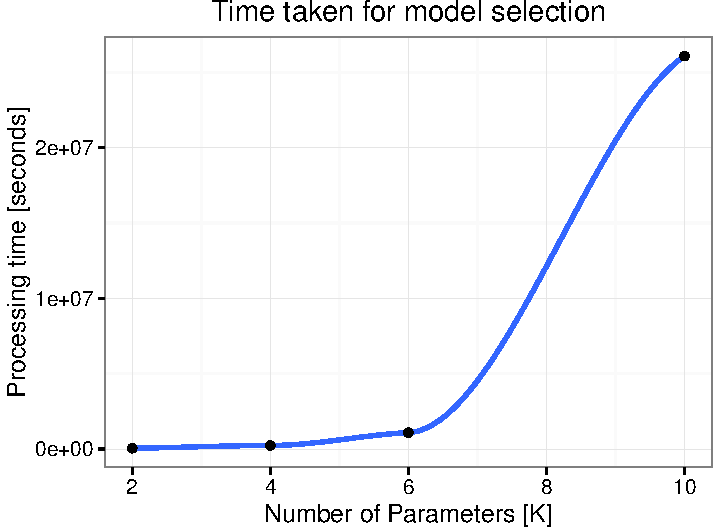
\includegraphics{diversityocc_files/figure-latex/unnamed-chunk-11-1} \end{center}

\end{CodeChunk}

From now on we will work with automatically selected models for bat
abundance and diversity using an information theoretic approach (AICc).

\begin{CodeChunk}
\begin{CodeInput}
batmodel.selected <- diversityoccu(pres = BatOccu, sitecov = sampling.cov, obscov = Dailycov,spp = 17, form = ~ Julian + Meanhum ~ Burn.intensity.soil + I(Burn.intensity.soil^2), dredge = TRUE)
\end{CodeInput}
\end{CodeChunk}

Below we present an example of an analysis with the full model (includes
all variables) and subsequently results from a model selection analysis,
both of them only for the second species:

\begin{CodeChunk}
\begin{CodeInput}
BatDiversity$models[[2]]
\end{CodeInput}
\begin{CodeOutput}

Call:
occuRN(formula = form, data = models[[i]])

Abundance:
                          Estimate     SE      z P(>|z|)
(Intercept)               0.000567 0.2829  0.002   0.998
Burn.intensity.soil       0.543374 0.3826  1.420   0.156
I(Burn.intensity.soil^2) -0.092936 0.0996 -0.933   0.351

Detection:
            Estimate    SE      z P(>|z|)
(Intercept)    0.113 0.357  0.317  0.7512
Julian        -0.097 0.267 -0.364  0.7159
Meanhum       -0.548 0.246 -2.228  0.0259

AIC: 180.113 
\end{CodeOutput}
\begin{CodeInput}
batmodel.selected$models[[2]]
\end{CodeInput}
\begin{CodeOutput}

Call:
occuRN(formula = ~Meanhum + 1 ~ Burn.intensity.soil + 1, data = data2)

Abundance:
                    Estimate     SE     z P(>|z|)
(Intercept)           0.0767 0.2637 0.291  0.7712
Burn.intensity.soil   0.1901 0.0973 1.953  0.0508

Detection:
            Estimate    SE      z P(>|z|)
(Intercept)    0.143 0.351  0.407  0.6840
Meanhum       -0.530 0.242 -2.190  0.0285

AIC: 177.0765 
\end{CodeOutput}
\end{CodeChunk}

The responses of individual species to specific variables can be shown
using the function respnseplot.abund, bellow we show the response of
abundance in species 2 to the Burn intensity soil. Note that this
function automatically bounds the limits of the variable to the maximum
and minimum observable values in the field.

\begin{CodeChunk}
\begin{CodeInput}
responseplot.abund(batmodel.selected, spp = 2, variable = Burn.intensity.soil)
\end{CodeInput}


\begin{center}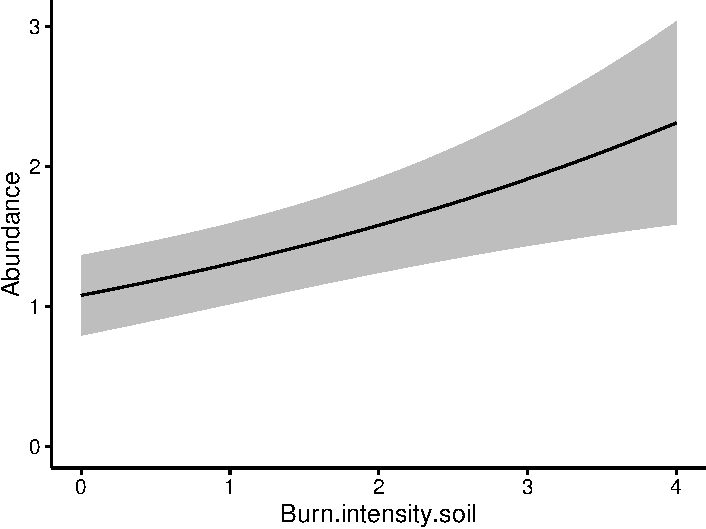
\includegraphics{diversityocc_files/figure-latex/unnamed-chunk-14-1} \end{center}

\end{CodeChunk}

\subsection{Model selection for alpha diversity
modeling}\label{model-selection-for-alpha-diversity-modeling}

\section{Discussion}\label{discussion}

The \pkg{DiversityOccupancy} package lets scientists and managers take
dessitions based on species information, diversity information or both.
In some countries, laws require that the decision is taken based on
endangered species information, the possibility on selecting an area, or
manage environments based on both diversity and species specific
information, gives a possibility to managers or decision makers wanting
to use diversity with laws requiring them to take species into account.

\end{document}

